\chapter{ĐẶT VẤN ĐỀ VÀ PHÂN TÍCH YÊU CẦU}

\section{Bối cảnh và mục tiêu}

\subsection{Bối cảnh bài toán}

Biển báo giao thông cung cấp cho người lái xe các thông tin về giới hạn tốc độ, cấm, cảnh báo nguy hiểm và chỉ dẫn. Một hệ thống hỗ trợ lái xe hoặc xe tự hành cần tự động nhận dạng loại biển trong ảnh chụp từ camera gắn trên xe. Bài toán khó ở chỗ cùng một loại biển có thể xuất hiện với kích thước rất khác nhau (biển ở xa chỉ vài chục điểm ảnh), trong nhiều điều kiện ánh sáng, và nhiều loại biển khác nhau chỉ khác ở chi tiết nhỏ, ví dụ chữ số trên các biển giới hạn tốc độ.

Bài tập lớn giải bài toán \textbf{phân loại ảnh biển báo giao thông vào 43 lớp}. Đầu vào là một ảnh biển báo, đầu ra là nhãn lớp \texttt{ClassId} nhận giá trị từ 0 đến 42. Nhóm chỉ sử dụng các thuật toán đã học trong học phần (K-NN và Cây quyết định), không dùng mạng nơ-ron.

\subsection{Mục tiêu và yêu cầu}

Theo hướng dẫn thực hiện bài tập lớn của học phần (Lê Thị Thùy Trang, 2026), nhóm đặt ra các mục tiêu sau:

\begin{itemize}
    \item Xây dựng quy trình học máy hoàn chỉnh từ dữ liệu thô đến kết quả đánh giá cuối cùng, có phương án baseline làm mốc so sánh.
    \item So sánh các cách biểu diễn đặc trưng (vector pixel, HOG, PCA) và các cách tiền xử lý (có hoặc không có CLAHE).
    \item So sánh hai thuật toán K-NN và Cây quyết định, khảo sát ảnh hưởng của các siêu tham số quan trọng (số láng giềng $k$, metric, độ sâu cây, tiêu chí chia).
    \item Chia dữ liệu đúng quy trình, các bước học tham số từ dữ liệu chỉ được học trên tập huấn luyện để hạn chế rò rỉ dữ liệu.
    \item Đánh giá bằng Accuracy, Precision, Recall, F1-score và ma trận nhầm lẫn; phân tích lớp dễ nhầm lẫn và các trường hợp dự đoán sai, không chỉ dựa trên Accuracy.
\end{itemize}

\section{Phân tích dữ liệu (EDA)}

\subsection{Nguồn dữ liệu}

Bộ dữ liệu sử dụng là German Traffic Sign Recognition Benchmark (GTSRB) (Stallkamp và cs., 2012), theo bản được đề bài chỉ định. Đường dẫn tải dữ liệu: \url{https://www.kaggle.com/datasets/meowmeowmeowmeowmeow/gtsrb-german-traffic-sign}. Dữ liệu không được đưa vào repository của nhóm vì dung lượng lớn (khoảng 500 MB).

\subsection{Cấu trúc dữ liệu}

Dữ liệu gồm các thư mục ảnh \texttt{Train/}, \texttt{Test/}, \texttt{Meta/} và ba tệp \texttt{Train.csv}, \texttt{Test.csv}, \texttt{Meta.csv}. Mỗi dòng của tệp CSV gồm 8 cột: \texttt{Width}, \texttt{Height}, bốn cột khung bao quanh biển \texttt{Roi.X1}, \texttt{Roi.Y1}, \texttt{Roi.X2}, \texttt{Roi.Y2}, nhãn \texttt{ClassId} và đường dẫn ảnh \texttt{Path}. Thư mục \texttt{Meta/} chứa 43 ảnh biển chuẩn (mỗi lớp một ảnh), chỉ dùng để tham khảo, không dùng để huấn luyện.

\begin{table}[H]
\centering
\caption{Thống kê tổng quan bộ dữ liệu}
\label{tab:thong-ke-du-lieu}
\begin{tabular}{|p{7cm}|p{7.5cm}|}
\hline
\textbf{Nội dung} & \textbf{Giá trị} \\
\hline
Số ảnh tập Train & 39\,209 \\
\hline
Số ảnh tập Test & 12\,630 \\
\hline
Số lớp (Train và Test) & 43 \\
\hline
Dữ liệu thiếu (Train, Test) & 0 \\
\hline
Đường dẫn ảnh trùng lặp (Train) & 0 \\
\hline
Lớp ít ảnh nhất & Lớp 0 (210 ảnh) \\
\hline
Lớp nhiều ảnh nhất & Lớp 2 (2\,250 ảnh) \\
\hline
Tỉ lệ mất cân bằng (lớn nhất/nhỏ nhất) & khoảng 10,7 lần \\
\hline
Số track trong tập Train & 1\,307 (khoảng 30 ảnh mỗi track) \\
\hline
Chiều rộng ảnh gốc (trung bình $\pm$ độ lệch chuẩn) & $50{,}8 \pm 24{,}3$ điểm ảnh \\
\hline
Chiều cao ảnh gốc (trung bình $\pm$ độ lệch chuẩn) & $50{,}3 \pm 23{,}1$ điểm ảnh \\
\hline
Kích thước nhỏ nhất, lớn nhất & $25$ điểm ảnh; $243 \times 225$ điểm ảnh \\
\hline
\end{tabular}
\Nguon{Nhóm tổng hợp từ tệp \texttt{results/eda\_summary.txt}}
\end{table}

\subsection{Phân phối lớp}

Dữ liệu \textbf{mất cân bằng}: lớp ít nhất có 210 ảnh, lớp nhiều nhất có 2\,250 ảnh (Hình~\ref{fig:phan-phoi-lop}). Vì vậy bên cạnh Accuracy, nhóm báo cáo thêm Macro-Precision, Macro-Recall và Macro-F1 (trung bình không trọng số trên 43 lớp) để các lớp ít ảnh không bị che lấp.

\begin{figure}[H]
    \centering
    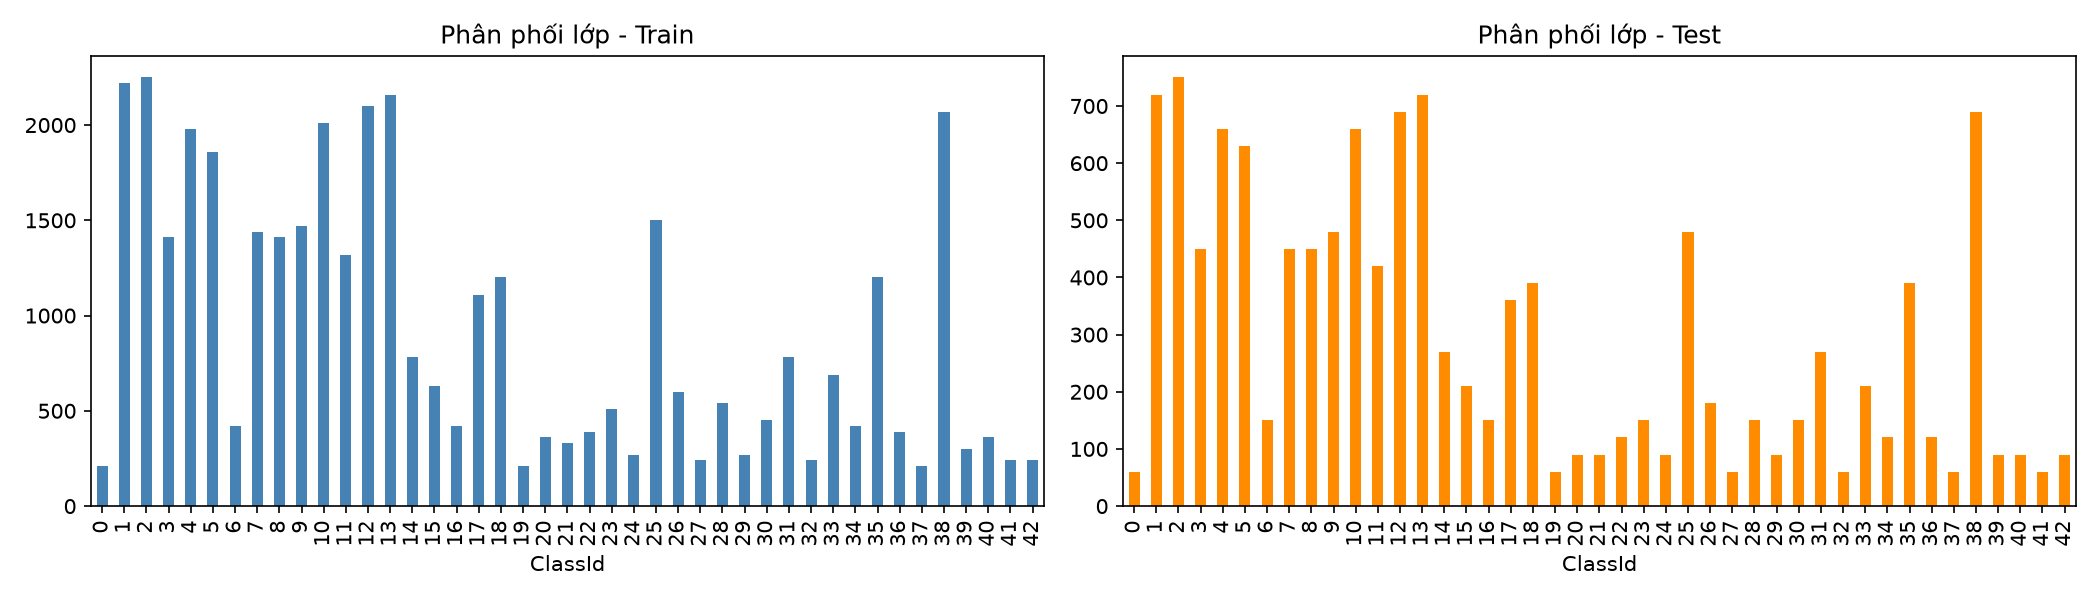
\includegraphics[width=\textwidth]{images/eda_class_distribution.png}
    \caption{Phân phối số ảnh theo lớp ở tập Train (trái) và Test (phải)}
    \label{fig:phan-phoi-lop}
    \Nguon{Nhóm vẽ từ bộ dữ liệu GTSRB}
\end{figure}

\subsection{Cấu trúc theo track và nguy cơ rò rỉ dữ liệu}

Ảnh trong GTSRB được chụp theo chuỗi: mỗi biển vật lý xuất hiện trong khoảng 30 khung hình liên tiếp, gọi là một \textit{track}. Tập Train có 1\,307 track. Các ảnh cùng track gần như giống hệt nhau. Nếu chia dữ liệu huấn luyện/kiểm định ngẫu nhiên theo từng ảnh, ảnh của cùng một biển sẽ nằm ở cả hai tập và kết quả kiểm định bị lạc quan giả tạo. Do đó nhóm chia theo track (mục~\ref{sec:chia-du-lieu}).

\subsection{Kích thước và độ sáng ảnh}

Ảnh có kích thước rất khác nhau: chiều rộng trung bình 50,8 điểm ảnh, trung vị 43, nhỏ nhất 25, lớn nhất 243 (Hình~\ref{fig:kich-thuoc}). Độ sáng trung bình của ảnh lệch về phía tối: phần lớn ảnh có độ sáng trung bình khoảng 20--120 trên thang 0--255, đỉnh quanh 50--70, và chỉ một số ít ảnh sáng trên 200 (Hình~\ref{fig:do-sang}). Quan sát này gợi ý bước cân bằng độ tương phản cục bộ (CLAHE) có thể hữu ích, đặc biệt với biểu diễn pixel; giả thuyết này được kiểm tra ở mục~\ref{sec:so-sanh-clahe}. Ảnh mẫu của từng lớp được trình bày ở Phụ lục 1.

\begin{figure}[H]
    \centering
    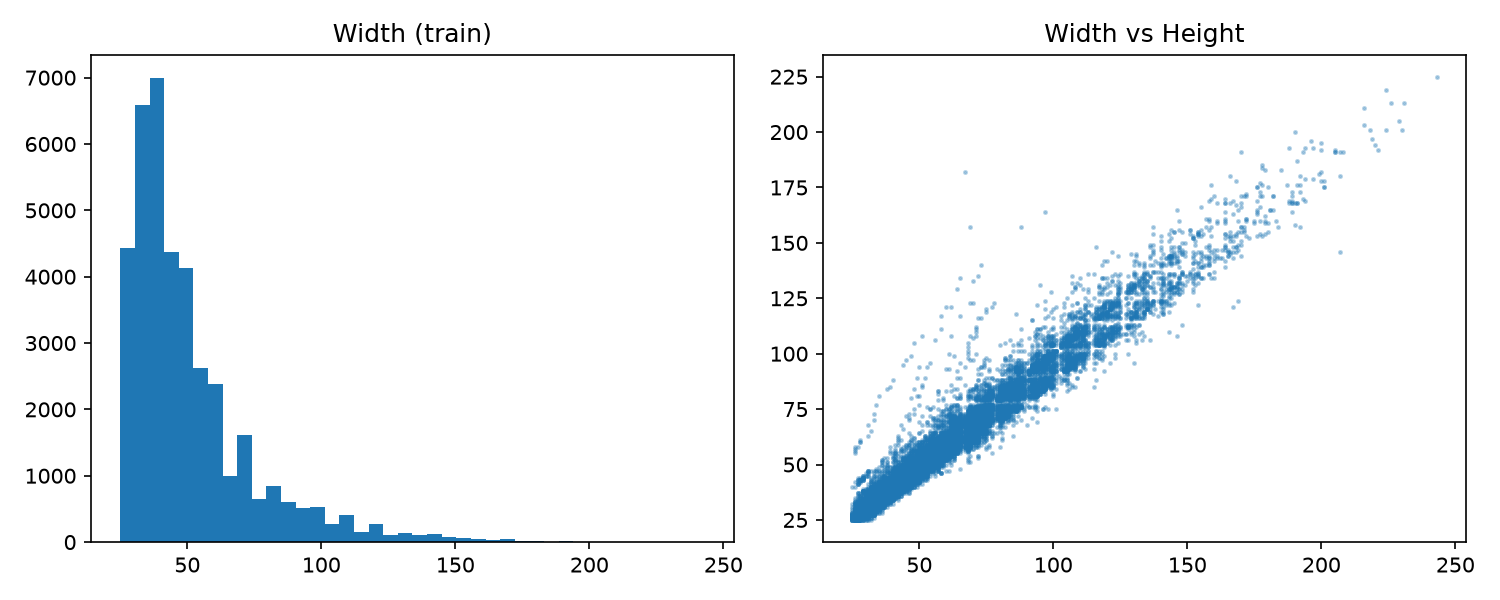
\includegraphics[width=0.85\textwidth]{images/eda_image_sizes.png}
    \caption{Phân bố kích thước ảnh gốc ở tập Train}
    \label{fig:kich-thuoc}
    \Nguon{Nhóm vẽ từ bộ dữ liệu GTSRB}
\end{figure}

\begin{figure}[H]
    \centering
    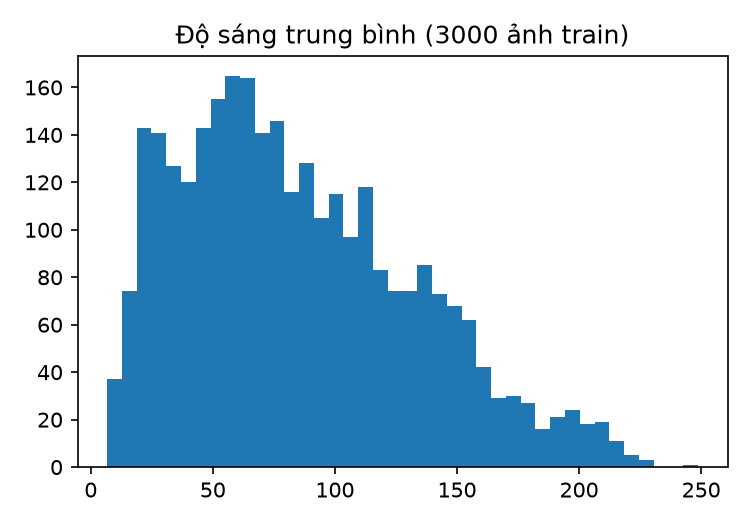
\includegraphics[width=0.6\textwidth]{images/eda_brightness.png}
    \caption{Phân bố độ sáng trung bình (3\,000 ảnh Train ngẫu nhiên)}
    \label{fig:do-sang}
    \Nguon{Nhóm vẽ từ bộ dữ liệu GTSRB}
\end{figure}
